\documentclass{article}

\usepackage[a4paper, total={7in, 10in}]{geometry}

\usepackage{hyperref}
\usepackage{amsmath}
\usepackage{subcaption}
\usepackage{parskip}
\usepackage{graphicx}
\graphicspath{{../Results/Protected/}}

\title{AIMS Course 1: Data, Estimation and Inference}
\author{Jake Levi}
\date{October 2022}

\begin{document}
\maketitle

% Section: introduction

\section{Introduction} \label{section:intro}

This lab report investigates the use of Gaussian Processes (GPs), a type of machine learning model motivated by Bayesian probability theory, for modelling a meteorological dataset called Sotonmet. In a GP model, given a mean function $\mu$, kernel function $K$, vaiance of observation noise $\sigma^2$, training inputs $x$ (represented as a vector), and prediction inputs $x^*$, the noisy training labels $y$ (which we assume are noisy observations of unknown labels $f$) and noiseless prediction labels $f^*$ have a joint Gaussian distribution:

% Equation: joint distribution

\begin{equation}
    p\left( \begin{bmatrix}
        y \\
        f^*
    \end{bmatrix} \right)
    = \mathcal{N} \left( \begin{bmatrix}
        y \\
        f^*
    \end{bmatrix} \middle| \begin{bmatrix}
        \mu(x) \\
        \mu(x^*)
    \end{bmatrix}, \begin{bmatrix}
        K(x, x) + \sigma^2 I & K(x, x^*) \\
        K(x, x^*)^T & K(x^*, x^*) \\
    \end{bmatrix} \right)
\end{equation}

Where $K(x, x^*)$ is a matrix whose $(i, j)$th element is given by $K(x, x^*)_{i,j} = K(x_i, x^*_j)$. The predictive distribution $p(f^* \mid y)$ follows from the formula for the conditional distribution of a jointly Gaussian random variable \cite{bishop2006pattern}:

% Equation: conditional distribution

\begin{align}
    p(f^* \mid y) &= \mathcal{N}\left(f^* \mid \mu^*, \Sigma^* \right) \label{eq:conditional distribution} \\
    \text{where} \quad \mu^* &= \mu(x^*) + K(x^*, x) \left( K(x, x) + \sigma^2 I \right)^{-1} (y - \mu(x)) \label{eq:conditional mean} \\
    \Sigma^* &= K(x^*, x^*) - K(x^*, x) \left( K(x, x) + \sigma^2 I \right) ^{-1} K(x, x^*) \label{eq:conditional variance}
\end{align}

The log marginal likelihood (LML) of the noisy training labels $y$ given training input data $x$ (and also implicitly given any hyperparameters of the model) is given by:

% Equation: log marginal likelihood

\begin{align}
    \log \left( p(y \mid x) \right) &= -\frac{1}{2}\log\left(\det \left(2\pi \Sigma_y \right)\right) -\frac{1}{2}(y - \mu(x))^T \Sigma_y^{-1} (y - \mu(x)) \\
    \text{where} \quad \Sigma_y &= K(x, x) + \sigma^2 I
\end{align}

This expression implies that maximising the LML encourages $\mu(x)$, $K(x,x)$ and $\sigma$ to fit the data accurately and with calibrated uncertainty. Maximising the LML can also be motivated from a Bayesian perspective, which is discussed further in Appendix \ref{appendix:why_lml}.

The focus in this coursework submission is on predicting the tide height given the time of day, for which the training and ground truth data is shown in figure \ref{fig:data}, alongside an independent GP prediction in figure \ref{fig:ind_pres}.

% Section: results

\section{Results}

We start off by considering GPs with constant mean function and squared exponential kernel, whose mean and kernel functions are related to the hyperparameters $c$, $k$, and $\lambda$ as follows ($\sigma$ is also considered to be a hyperparameter, although it is not explicitly part of the mean or kernel functions):

% Equation: constant mean and squared exponential kernel function

\begin{align}
\mu(x) &= c \\
K_{\mathrm{sqe}}(x, x') &= k \exp\left( -\left( \frac{x - x'}{\lambda} \right)^2 \right)
\end{align}

Initially we consider two GPs denoted by sqe\_1 and sqe\_2, whose hyperparameter values are described in table \ref{table:sqe_hyperparameters}. Samples from the prior distributions of sqe\_1 and sqe\_1 are shown in figures \ref{fig:prior_sqe_1} and \ref{fig:prior_sqe_2}, which show that the prior distribution of sqe\_1 looks subjectively like a much more plausible explanation for the data. The predictive distributions of these GPs are shown in figures \ref{fig:pred_dist_sqe_1} and \ref{fig:pred_dist_sqe_2}, which show that, although sqe\_1 produced a \emph{prior} distribution which looks like a more plausible explanation for the training data, sqe\_2 produces a \emph{predictive} distribution which looks like a much better fit to the training data. Furthermore, the predictive distribution of sqe\_1 is "confidently wrong" (the mean is far away from the ground truth labels and with high certainty/low standard deviation) in regions containing ground truth labels but no training data, which would be a very undesirable property of a machine learning prediction model in a safety-critical context. Samples from the predictive distribution of both GPs are shown in figures \ref{fig:pred_samples_sqe_1} and \ref{fig:pred_samples_sqe_2}, which show that neither GP produces samples that reflect the data distribution particularly well.

The evaluation of GPs sqe\_1 and sqe\_2 according to the metrics RMSE (square root of the mean-squared-error between labels and the GP's predictive mean), LML, and log predictive likelihood (LPL, which is just the logarithm of equation \ref{eq:conditional distribution} given the expression for a multivariate Gaussian probability density function \cite{bishop2006pattern}), is summarised in table \ref{table:sqe_metrics}. Note that although sqe\_1 has a very low RMSE evaluated on the training data, it has an RMSE which is $30\times$ higher when evaluated on the ground truth data, which is to say that sqe\_1 overfits the training data very badly, which is reflected in its relatively bad LML and LPLs. sqe\_2 has worse RMSE on the training data than the sqe\_1, but better RMSE on the ground truth data, which is to say that sqe\_2 generalises better to unseen data (although it does so with low confidence/high uncertainty, as seen in sqe\_2's predictive samples in figure \ref{fig:pred_samples_sqe_2}), and this is reflected in the better LML and LPLs of sqe\_2.

As mentioned in section \ref{section:intro}, the LML can be used as an objective function to optimise the hyperparameters of a GP. Starting with sqe\_2 (because this GP has greater LML than sqe\_1), the parameters of this GP can be optimised using the L-BFGS-B algorithm \cite{wright1999numerical}, leading to a GP referred to as sqe\_opt, whose hyperparameter values and evaluation metrics are described in table \ref{table:sqe}. Remarkably, sqe\_opt has worse RMSE on training data than sqe\_1, but better RMSE on ground truth data. This implies that optimising RMSE on training data (which is often performed in machine learning) is not always a good approach, because an improvement in the RMSE on training data might lead to decreased predictive performance on unseen data, which is generally of greater importance in machine learning.

\appendix

% Figure: Sotonmet dataset

\begin{figure}[pht]
    \centering
    \subfloat[
        \centering Training and ground truth data
        \label{fig:data}
    ]{
        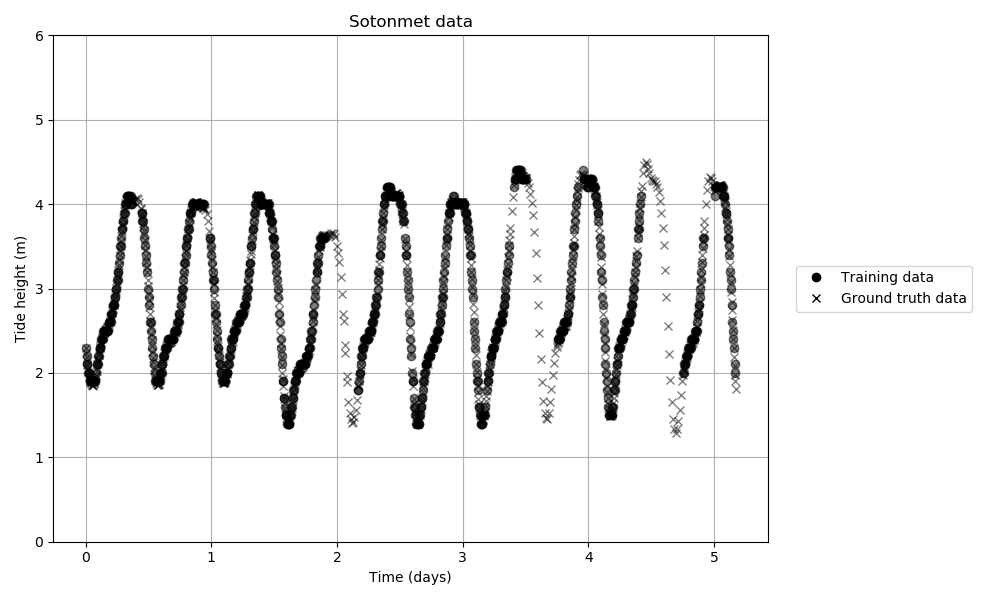
\includegraphics[width=0.45\textwidth]{Sotonmet_data.png}
    }
    \subfloat[
        \centering Independent GP predictions
        \label{fig:ind_pres}
    ]{
        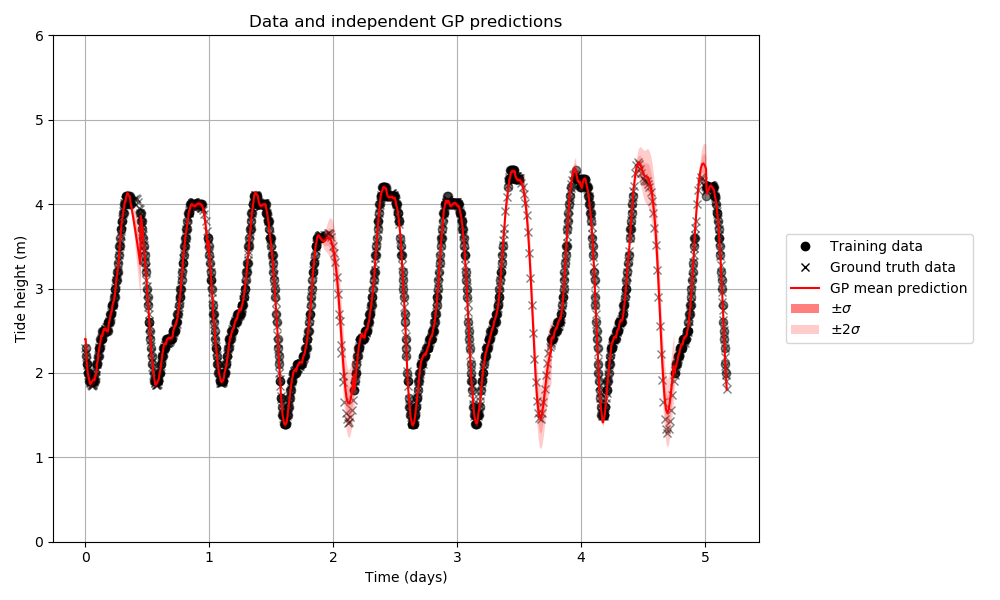
\includegraphics[width=0.45\textwidth]{Data_and_independent_GP_predictions.png}
    }
    \caption{The Sotonmet dataset}
    \label{fig:sotonmet}
\end{figure}

% Figure: GPs with SQE kernel

\begin{figure}[pht]
    \centering
    \begin{subfigure}{0.45\textwidth}
        \centering
        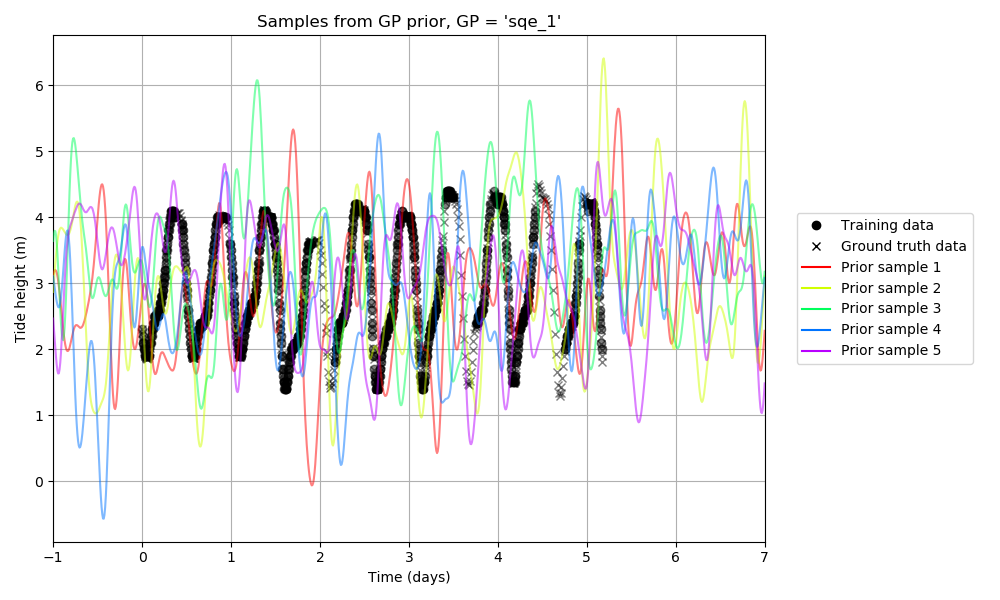
\includegraphics[width=\textwidth]{Samples_from_GP_prior,_GP____sqe_1_.png}
        \caption{Samples from the prior of sqe\_1}
        \label{fig:prior_sqe_1}
    \end{subfigure}
    \begin{subfigure}{0.45\textwidth}
        \centering
        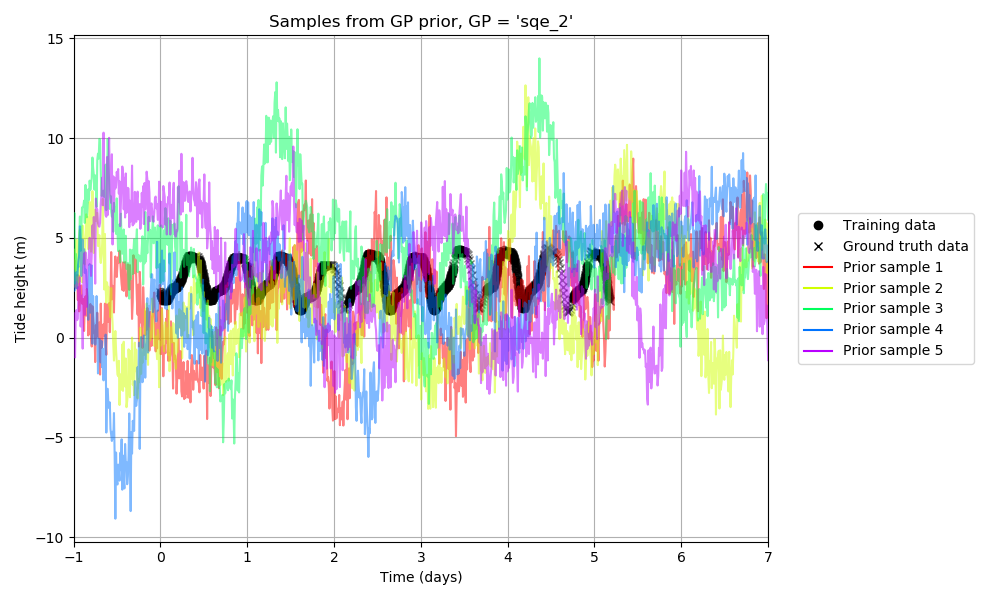
\includegraphics[width=\textwidth]{Samples_from_GP_prior,_GP____sqe_2_.png}
        \caption{Samples from the prior of sqe\_2}
        \label{fig:prior_sqe_2}
    \end{subfigure}
    \newline
    \begin{subfigure}{0.45\textwidth}
        \centering
        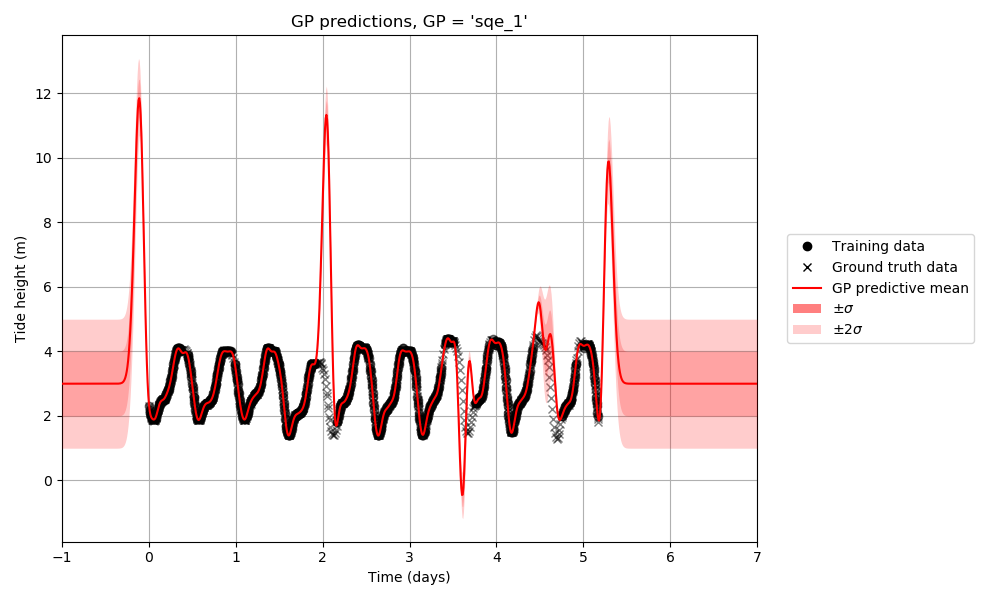
\includegraphics[width=\textwidth]{GP_predictions,_GP____sqe_1_.png}
        \caption{Predictive distribution of sqe\_1}
        \label{fig:pred_dist_sqe_1}
    \end{subfigure}
    \begin{subfigure}{0.45\textwidth}
        \centering
        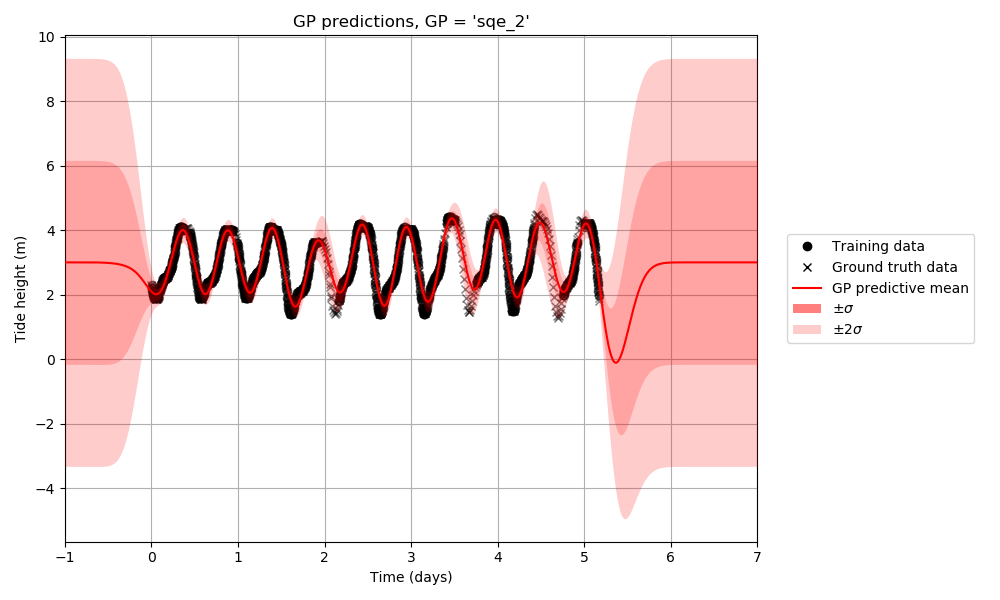
\includegraphics[width=\textwidth]{GP_predictions,_GP____sqe_2_.png}
        \caption{Predictive distribution of sqe\_2}
        \label{fig:pred_dist_sqe_2}
    \end{subfigure}
    \newline
    \begin{subfigure}{0.45\textwidth}
        \centering
        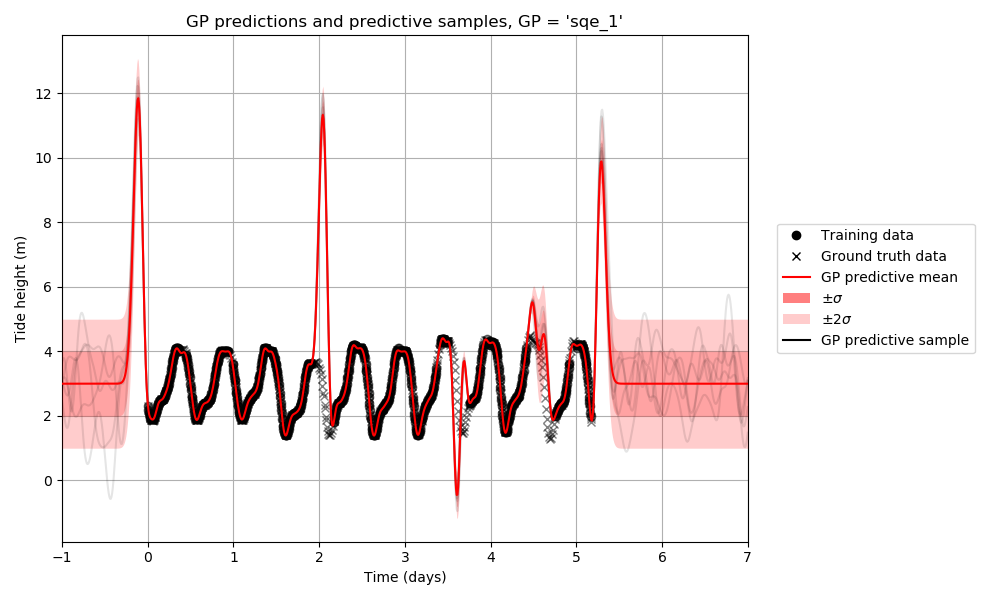
\includegraphics[width=\textwidth]{GP_predictions_and_predictive_samples,_GP____sqe_1_.png}
        \caption{Samples from the predictive distribution of sqe\_1}
        \label{fig:pred_samples_sqe_1}
    \end{subfigure}
    \begin{subfigure}{0.45\textwidth}
        \centering
        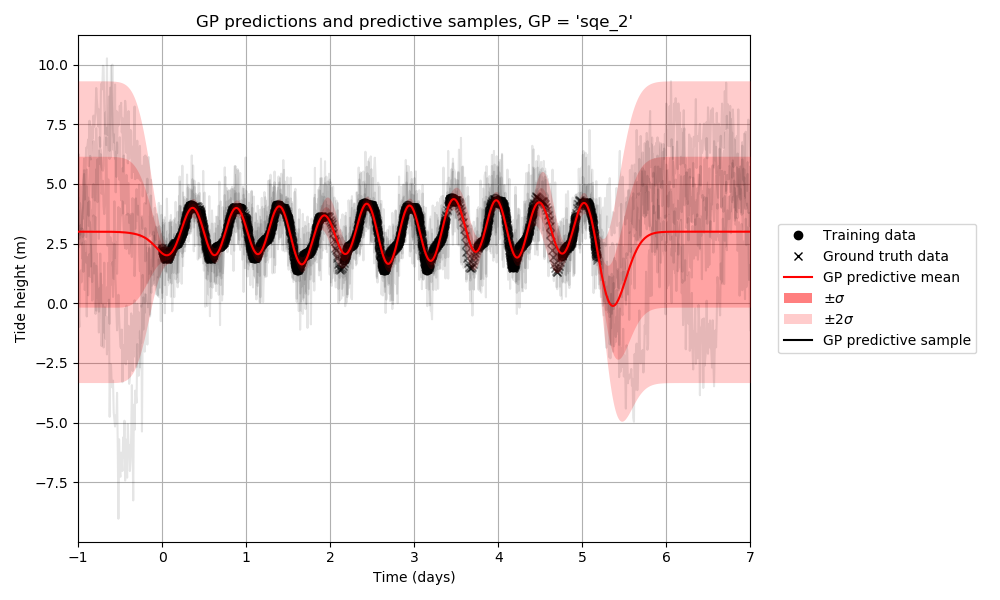
\includegraphics[width=\textwidth]{GP_predictions_and_predictive_samples,_GP____sqe_2_.png}
        \caption{Samples from the predictive distribution of sqe\_2}
        \label{fig:pred_samples_sqe_2}
    \end{subfigure}

    \caption{Prior and predictive distributions of GPs with square exponential kernels}
    \label{fig:sqe}
\end{figure}

% Table: SQE GPs

\begin{table}[ht]
    \centering
    \begin{subtable}[t]{0.45\textwidth}
        \centering
        \begin{tabular}[t]{|c|c|c|c|}
            \hline
            Hyperparameter & sqe\_1 & sqe\_2 & sqe\_opt \\
            \hline
            $c$ & 3.0000 & 3.0000 & 2.9905 \\
            $\lambda$ & 0.1000 & 0.3000 & 0.0867 \\
            $k$ & 1.0000 & 10.0000 & 0.6522 \\
            $\sigma$ & 0.0010 & 1.0000 & 0.0293 \\
            \hline
        \end{tabular}
        \caption{}
        \label{table:sqe_hyperparameters}
    \end{subtable}
    \begin{subtable}[t]{0.45\textwidth}
        \centering
        \begin{tabular}[t]{|c|c|c|c|}
            \hline
            Metric & sqe\_1 & sqe\_2 & sqe\_opt \\
            \hline
            RMSE (train) & 0.0268 & 0.2246 & 0.0275 \\
            RMSE (truth) & 0.8040 & 0.2573 & 0.1587 \\
            LML & -327743.8 & -942.0 & 1574.4 \\
            LPL (train) & -321611.9 & -875.4 & 1954.9 \\
            LPL (truth) & -87596.3 & -894.3 & 3366.3 \\
            \hline
        \end{tabular}
        \caption{}
        \label{table:sqe_metrics}
    \end{subtable}
    \caption{\ref{table:sqe_hyperparameters} Values of the hyperparameters of 3 GPs with squared exponential kernels that are considered in this report, \ref{table:sqe_metrics} their evaluation according to different metrics}
    \label{table:sqe}
\end{table}

\section{Motivation for maximising the log marginal likelihood}\label{appendix:why_lml}

% References and end of document

\bibliographystyle{plain}
\bibliography{references}

\end{document}
